\documentclass[12pt,twoside]{report}

%%%%%%%%%%%%%%%%%%%%%%%%%%%%%%%%%%%%%%%%%%%%%%%%%%%%%%%%%%%%%%%%%%%%%%%%%%%%%

% Definitions for the title page
% Edit these to provide the correct information
% e.g. \newcommand{\reportauthor}{Timothy Kimber}

\newcommand{\reporttitle}{Dynamics of Social Networks}
\newcommand{\reportauthor}{John Freeman}
\newcommand{\supervisor}{Alex Carver}
\newcommand{\degreetype}{Computing - Specialism}

\usepackage{float}

\usepackage{xcolor}
\setcounter{tocdepth}{2}

%%%%%%%%%%%%%%%%%%%%%%%%%%%%%%%%%%%%%%%%%%%%%%%%%%%%%%%%%%%%%%%%%%%%%%%%%%%%%

% load some definitions and default packages
%%%%%%%%%%%%%%%%%%%%%%%%%%%%%%%%%%%%%%%%%
% University Assignment Title Page 
% LaTeX Template
% Version 1.0 (27/12/12)
%
% This template has been downloaded from:
% http://www.LaTeXTemplates.com
%
% Original author:
% WikiBooks (http://en.wikibooks.org/wiki/LaTeX/Title_Creation)
%
% License:
% CC BY-NC-SA 3.0 (http://creativecommons.org/licenses/by-nc-sa/3.0/)
% 
%
%%%%%%%%%%%%%%%%%%%%%%%%%%%%%%%%%%%%%%%%%
%----------------------------------------------------------------------------------------
%	PACKAGES AND OTHER DOCUMENT CONFIGURATIONS
%----------------------------------------------------------------------------------------
\usepackage[a4paper,hmargin=2.8cm,vmargin=2.0cm,includeheadfoot]{geometry}
\usepackage{textpos}
\usepackage{natbib} % for bibliography
\usepackage{tabularx,longtable,multirow,subfigure,caption}%hangcaption
\usepackage{fncylab} %formatting of labels
\usepackage{fancyhdr} % page layout
\usepackage{url} % URLs
\usepackage[english]{babel}
\usepackage{amsmath}
\usepackage{algorithm}
\usepackage[noend]{algpseudocode}
\usepackage{graphicx}
\usepackage{dsfont}
\usepackage{epstopdf} % automatically replace .eps with .pdf in graphics
%\usepackage{backref} % needed for citations
\usepackage{array}
\usepackage{latexsym}
\usepackage[pdftex,hypertexnames=false,colorlinks]{hyperref} % provide links in pdf

\hypersetup{pdftitle={},
  pdfsubject={}, 
  pdfauthor={},
  pdfkeywords={}, 
  pdfstartview=FitH,
  pdfpagemode={UseOutlines},% None, FullScreen, UseOutlines
  bookmarksnumbered=true, bookmarksopen=true, colorlinks,
    citecolor=black,%
    filecolor=black,%
    linkcolor=black,%
    urlcolor=black}

%\usepackage[all]{hypcap}


%\usepackage{color}
%\usepackage[tight,ugly]{units}
%\usepackage{float}
%\usepackage{tcolorbox}
%\usepackage[colorinlistoftodos]{todonotes}
% \usepackage{ntheorem}
% \theoremstyle{break}
% \newtheorem{lemma}{Lemma}
% \newtheorem{theorem}{Theorem}
% \newtheorem{remark}{Remark}
% \newtheorem{definition}{Definition}
% \newtheorem{proof}{Proof}


%%% Default fonts
\renewcommand*{\rmdefault}{bch}
\renewcommand*{\ttdefault}{cmtt}



%%% Default settings (page layout)
\setlength{\parindent}{0em}  % indentation of paragraph

\setlength{\headheight}{14.5pt}
\pagestyle{fancy}
\renewcommand{\chaptermark}[1]{\markboth{\chaptername\ \thechapter.\ #1}{}} 

\fancyfoot[ER,OL]{\sffamily\textbf{\thepage}}%Page no. in the left on odd pages and on right on even pages
\fancyfoot[OC,EC]{\sffamily }
\renewcommand{\headrulewidth}{0.1pt}
\renewcommand{\footrulewidth}{0.1pt}
\captionsetup{margin=10pt,font=small,labelfont=bf}


%--- chapter heading

\def\@makechapterhead#1{%
  \vspace*{10\p@}%
  {\parindent \z@ \raggedright \sffamily
    \interlinepenalty\@M
    \Huge\bfseries \thechapter \space\space #1\par\nobreak
    \vskip 30\p@
  }}

%---chapter heading for \chapter*  
\def\@makeschapterhead#1{%
  \vspace*{10\p@}%
  {\parindent \z@ \raggedright
    \sffamily
    \interlinepenalty\@M
    \Huge \bfseries  #1\par\nobreak
    \vskip 30\p@
  }}

%\allowdisplaybreaks

% load some macros
% Here, you can define your own macros. Some examples are given below.

\newcommand{\R}[0]{\mathds{R}} % real numbers
\newcommand{\Z}[0]{\mathds{Z}} % integers
\newcommand{\N}[0]{\mathds{N}} % natural numbers
\newcommand{\C}[0]{\mathds{C}} % complex numbers
\renewcommand{\vec}[1]{{\boldsymbol{{#1}}}} % vector
\newcommand{\mat}[1]{{\boldsymbol{{#1}}}} % matrix


\date{September 2019}

\begin{document}

% load title page
% Last modification: 2015-08-17 (Marc Deisenroth)
\begin{titlepage}

\newcommand{\HRule}{\rule{\linewidth}{0.5mm}} % Defines a new command for the horizontal lines, change thickness here


%----------------------------------------------------------------------------------------
%	LOGO SECTION
%----------------------------------------------------------------------------------------


\includegraphics[width = 4cm]{./figures/imperial}\\[0.5cm] 

\center % Center remainder of the page

%----------------------------------------------------------------------------------------
%	HEADING SECTIONS
%----------------------------------------------------------------------------------------

\textsc{\Large Imperial College London}\\[0.5cm] 
\textsc{\large Department of Computing}\\[0.5cm] 

%----------------------------------------------------------------------------------------
%	TITLE SECTION
%----------------------------------------------------------------------------------------

\HRule \\[0.4cm]
{ \huge \bfseries \reporttitle}\\ % Title of your document
\HRule \\[1.5cm]
 
%----------------------------------------------------------------------------------------
%	AUTHOR SECTION
%----------------------------------------------------------------------------------------

\begin{minipage}{0.4\textwidth}
\begin{flushleft} \large
\emph{Author:}\\
\reportauthor % Your name
\end{flushleft}
\end{minipage}
~
\begin{minipage}{0.4\textwidth}
\begin{flushright} \large
\emph{Supervisor:} \\
\supervisor % Supervisor's Name
\end{flushright}
\end{minipage}\\[4cm]


%----------------------------------------------------------------------------------------
%	FOOTER & DATE SECTION
%----------------------------------------------------------------------------------------
\vfill % Fill the rest of the page with whitespace
Submitted in partial fulfillment of the requirements for the MSc degree in
\degreetype~of Imperial College London\\[0.5cm]

\makeatletter
\@date 
\makeatother


\end{titlepage}



% page numbering etc.
\pagenumbering{roman}
\clearpage{\pagestyle{empty}\cleardoublepage}
\setcounter{page}{1}
\pagestyle{fancy}

%%%%%%%%%%%%%%%%%%%%%%%%%%%%%%%%%%%%
\begin{abstract}

Ever since the first online social networks were constructed, people have sought to understand and influence them for reasons as diverse as basic research and advertising. These early primitive social networks have rapidly evolved into the massive behemoths we know today, connecting almost 40\% of the global population. As the networks grow in importance, so too does our desire to understand their characteristics. That growth in importance also correlates with a growth in intractability: the techniques of a decade ago couldn't possibly cope with the massive data we are immersed in today. \\

Seizing upon this challenge, we set out to create two systems to better understand online social networks: a dynamic network model and a dynamic node embedding system. Drawing from existing literature, we synthesize a model composed primarily of three others: the Apt-Markakis model of product diffusion, the Schelling model of segregation, and the Barabási–Albert model of preferential attachment. Using that model as a synthetic data generation tool, we develop a graph-convolutional autoencoder to embed graphs into a vector space that we go on to show is more effective than other existing models. \\

We demonstrate several emergent properties of our network model: weak scale-free structure, weak self-similarity, small-world characteristics, densification, and high modularity. To our knowledge such a study has not been done on Schelling networks in a dynamic context and as such we view the densification as especially interesting given it is a direct result of the Schelling process in our model. \\

We test our graph embedding system against two other embedding systems, one static and one dynamic. While our embedding quality was typically worse than retraining the static system at each time step, we consistently outperformed the reference dynamic embedding system on both clustering performance and stability. In terms of running time, our model tends to take longer on small datasets due to large overhead, but begins to outperform the others the larger the dataset. \\

\end{abstract}

\cleardoublepage
%%%%%%%%%%%%%%%%%%%%%%%%%%%%%%%%%%%%

\section*{Acknowledgments}

None of the work accomplished here would have been possible without a long list of people I have known or been influenced by these past 22 years. I cannot hope to list all the giants on whose shoulders I stand but I would like to make some acknowledgments regardless. \\

To Alex Carver, for supervising this project and invaluable mentoring along the way.

To all the professors and teachers that have taught me almost all I know.

To all the researchers I cite for laying the groundwork for what I accomplish here.

To all my friends for keeping me sane and being great companions. 

To my family, without whom I couldn't hope to be where I am today.\\
 
To all these people I extend my sincerest thanks. \\

\clearpage{\pagestyle{empty}\cleardoublepage}

%%%%%%%%%%%%%%%%%%%%%%%%%%%%%%%%%%%%
%--- table of contents
\fancyhead[RE,LO]{\sffamily {Table of Contents}}
\tableofcontents 


\clearpage{\pagestyle{empty}\cleardoublepage}
\pagenumbering{arabic}
\setcounter{page}{1}
\fancyhead[LE,RO]{\slshape \rightmark}
\fancyhead[LO,RE]{\slshape \leftmark}

%%%%%%%%%%%%%%%%%%%%%%%%%%%%%%%%%%%%
\chapter{Introduction}

The world has always been composed of networks. From the simplest intracellular protein networks to the most complex continent-spanning ecosystems, almost all real-world phenomena are results of smaller networks or components of larger ones. While these real-world networks have been and continue to be difficult to study due to the difficulty of collecting good data, the advent of the information age has led to the emergence of new classes of human designed and built networks that are inherently easier to study. \\

Foremost amongst this new class of human designed networks is the online social network, typified by the likes of Facebook or Twitter or Instagram. Within these networks we have a treasure trove of information at our fingertips: with the touch of a button we can collect megabytes of metadata ranging from favorite songs and foods to lists of friends. While the former may be of interest to those seeking to advertise or influence, we restrict ourselves to the latter, as indeed network topology is itself an expression of the preferences of its users, as shown by Centola \cite{centola2015social}.\\

No matter what a given online social network allows or encourages its users to share about themselves they have one thing in common: network structure. We can view each user in the network as a node: each connected by edges to those other users they interact with. The result of applying this to all the users of the network gives rise to the network's topology: the vast non-Euclidean substrate that users are embedded in. This topology is not static however: it is a swirling, ever-evolving thing whose structure and properties could change dramatically with as simple a change as the end of a friendship. \\

The scale of these networks is vast. At the time of writing Facebook alone has 2.3 billion registered users, each of which has an average of 338 friends. The underlying graph of Facebook then has 388.7 billion edges, an already a near-incomprehensible magnitude made worse by the knowledge that the network can only truly be understood as a time series, ever changing and ever-evolving on a scale that can only be fully captured at intervals of fractions of seconds. The task of analyzing the entirety of such a network is intractable for almost all useful tasks: even should NP be shown to be equivalent to P the amount of distributed computing power needed to even load that data into memory is astronomical. \\

Given the scale of these networks it is prudent to ask what we can gain from their analysis. To this question there are a myriad of answers: from targeted advertising to influence maximization to broader questions such as understanding how human interactions give rise to complex phenomena and how it relates to the interactions of other systems. We live in a modern, data-driven world where knowledge of these phenomena and how to exploit them increasingly can have a major impact on the world at large. It is as such imperative to develop systems and methods that give us a deep understanding of networks to both meet the needs of those who seek to influence networks are good, and know when others are doing so for more nefarious reasons. \\

The only way we can hope to understand such networks is thus through models. We know basic properties shared throughout social networks in general ranging from how their degree distributions are structured to how their shortest paths are expected to behave. We can replicate these properties on a smaller scale through a plethora of models that have been proposed. Once these models have captured the dynamics and characteristics of their real-world counterparts, we can safely use them to create new methods of network analysis, in our case that of network embeddings. \\

Graph and network theoretic problems have an unfortunate tendency to reside in NP class, stemming in no small part from their non-Euclidean structure. This poses an obvious solution: mapping the networks to a vector space. Such a task is a highly non-convex optimization problem, an area that until the advent of neural networks was itself near-intractable. The process of solving that problem is today known as graph embedding, and is increasingly becoming a major part of social network analytics. After all, why waste time designing complex approximation algorithms for situation-specific tasks when you can generate an embedding and apply standard tools from statistics and machine learning? \\

The modern world is awash in data, more data than we could hope to analyze. In this project however, we will be creating two systems that should make that task ever so slightly easier: a dynamic model of social networks capturing dynamics over time, and a graph embedding system to translate graphs into a vector space. \\

%%%%%%%%%%%%%%%%%%%%%%%%%%%%%%%%%%%%
\chapter{Background}

Our project is based off of research primarily in graph theory, social network modeling, and neural networks. Here we discuss the antecedents of our work outside of those basics: specifically some specific network models and graph convolutional networks. \\

\section{Networks and Models} 

We can describe a social network as a simple undirected graph $G$, composed of some edges $E$ and some vertices or nodes $V$. In general, the vertices of a social network correspond to the individuals or entities that inhabit it. The edges have more variance in what they can represent, but in general and in our case denote a 
$friend$ or $follow$ relation, a trivial example being an edge exists between two people $u$ and $v$ if they are friends in the given network. \\

Many models have been put forward to simulate the behavior we see in real-world networks, social or otherwise. We will be combining three models in this paper to try to build a comprehensive model of a social network: the Apt-Markakis model of product adoption, the Schelling model of self-segregation, and the Barabási–Albert model of scale-freeness. Each of these three models simulates a different aspect of social networks we hope to capture: Apt-Markakis handling opinion spread, Schelling handling community formation, and Barabási–Albert keeping the network dynamic and scale-free. \\

\subsection{Diffusion and Organization}

Modeling static networks can readily be done through simple graph-theoretic and geometric techniques, and such techniques can generate representative static graphs easily, indeed many of them can produce graphs near exactly mimicking real-world network properties, as exemplified by Wu et al \cite{wu2015emergent}. Such models do have a major drawback however: the networks evolution over time is often not nearly as representative of the real-world as their final states. \\

We can overcome that issue by utilizing two properties seen in real-world graphs themselves: diffusion and self-organization. Diffusion refers to the process of information spreading across a network, and can be intuitively be understood as people sharing a piece of news until it reaches everyone in the network. Diffusion is a deeply complex process that is difficult to capture the entirety of, but it is likewise critical in understanding real network evolution. Again, we can intuitively imagine a case where a friend $u$ sees a piece of news shared by their friend $v$ originating from a third party $w$, we could expect $u$ to be more likely to form a friendship with $w$ as opposed to another random user. \\

Self-organization is more self-explanatory, referring to the process by which a structured network topology emerges as a consequence of the interactions of its users. This can take on many, many different forms, and the task of even discovering whether a network is organizing can be difficult in and of itself. That being said, organization again has an intuitive basis: we'd expect a group of real-world friends to have more friendship links within their group than outside, and a repetition of that structure across an entire network leads to what in graph theory we refer to as communities. One case of self-organization is self-segregation, which is what we will attempt to simulate. Self-segregation is simply the idea that people more prefer to be friends with those similar to them, and prefer not to be friends with those dissimilar, within some tolerances. Again, repeating this behavior across all users in a network can lead to complex emergent topologies in much the same manner. \\

\subsection{Apt and Markakis's Model}

The Apt-Markakis model \cite{apt2011diffusion} was designed to model the diffusion of products across a social network. In the simplest case, each node is initialized to have either adopted a product, or a threshold at which it will adopt one. The model then continuously checks nodes that have not adopted products to see if the fraction of its neighbors that have adopted a given product exceeds the node's threshold. If a node's threshold is met, it adopts the most common product of its neighbors. Apt and Markakis go on to show numerous results of computational complexity of various problems on their model, but the aspect of it we take advantage of in this project is its ability to easily model product, or in our case opinion, diffusion across a network. \\

\subsection{Schelling's Model}

A natural synergy with the Apt-Markakis model is Schelling's model of self-segregation \cite{schelling1971dynamic}. In Schelling's model, nodes evaluate whether they are satisfied in their location or not by checking how many dissimilar neighbors they have. Should a node be dissatisfied, it will move to a neighborhood that is more similar to itself, again according to dissimilarity thresholds. Schelling's model has been extensively studied and has been shown to accurately characterize many more real-world behaviors than those put forwards in his paper. It is especially useful to us as it provides a mechanism to make our model dynamic, with connections being made and broken according to node opinions and tolerances. \\

\subsection{Barabási and Albert's Model}

A common if not ubiquitous characteristic of real-world networks is scale-freeness, a term used to describe graphs with log-linear degree distributions. Many models have been put forwards to create networks with this property, but arguably the most popular is the Barabási–Albert model \cite{barabasi1999emergence}. In the model, we start with an initial graph and continuously add nodes to it. At each addition, we calculate the probability an edge exists between it and a given node in the graph by the proportion of its degree to the total degree of the graph. This simulates a "rich get richer" system where nodes with higher degree will have their degrees increase faster than those with lower degree, which in turn yields a scale-free network. \\

\subsection{Properties of Real Networks}

There are several emergent characteristics endemic to real-world networks that we hope to capture through our synthetic model, all of which have been seen in real-world networks ranging from the Internet to protein interaction networks to social media: scale-free, small world \cite{wang2003complex}, and self-similar structures \cite{song2005self}. \\

\subsection{Scale-Free Networks}
A network is said to be scale-free if the degrees of its nodes follow a power law: effectively meaning that few nodes have many connections, and many nodes have few connections. While this property seems at first glance inconsequential, this property is thought to characterize many real-world networks, and as such is an important property to capture if our model is to be representative.  \\

\subsection{Small-World Networks}
Closely related to scale-free networks, small-world networks have a less well accepted definition, but common metrics include diameter increasing at most logarithmically with network size, or higher clustering but equivalent average path length compared to random networks. Effectively, what those metrics capture is classic idea of six degrees of seperation, that all people on Earth are at most 6 friends away from each other. As the precise definition of small-world networks varies, and measuring large real-world networks for such metrics as average path length and diameter are computationally intensive, the classification of real-world networks as small-world varies by person to person, but it is generally accepted that most social networks fall into this category \cite{telesford2011ubiquity}. \\

\subsection{Self-Similar Networks}
A less well known and studied property of networks is self-similarity. As the name suggests, self-similarity is the network equivalent of fractal structure in geometric space. As with fractals, a network is self-similar if it is length-scale invariant, meaning as in fractals, the structure of the network is the same no matter how zoomed in you look at it. \\

While zooming in on a geometric structure is of course trivial, the generalization to networks is not as difficult as one might imagine, and is done through a process known as renormalization \cite{song2005self}. Renormalization is similar to the standard box-counting method, where the network is segmented into boxes corresponding to the neighborhoods of randomly selected nodes with a predetermined radius, and then collapsed down so that the boxes are nodes. It has been shown that for many networks, including the http-level Internet, properties of the graphs stay the same after renormalization, most notably in the case of the Internet, the degree distribution remains scale-free. \\

\section{Machine Learning on Graphs}

Traditionally, graph theoretic problems have been addressed through mathematical and computer scientific approaches, with complexity classes being extensively studied and approximation algorithms being created to deal with the NP-completeness that is pervasive in graph-based problems. While such approaches are generally successful, modern data-driven methodologies have become increasingly common in the analysis of graphs, especially on large real-world datasets. \\

Machine learning type algorithms have arrived relatively late to graph problems, in a large part due to the dissimilarity of the data to other approaches. Most algorithms rely on input vectors of numerical data and have few ways of efficiently representing topological information of the graphs themselves, often forcing them to resort to using node attributes augmented by simple human made features. Worse still is the case of unattributed nodes where the topology of the network is all that can be learned from, where algorithms are reduced to considering adjacency information alone. While attribute information is no doubt useful, the topology of the graph often contains more useful information, especially for graph theoretic problems. \\ 

\subsection{Graph Embedding}

A common way of applying machine learning techniques to graphs is to create a graph embedding, that is, mapping the nodes of a graph into a vector space. Many techniques exist for this: initially spectral methods based off adjacency matrices and other information, and later based off random walks and eventually deep learning methods on the graph itself. The key in graph embeddings is to find a representation vector for a given node such that the structural and attribute properties of the graph are preserved in the embedding space. \\

The problem of graph embeddings has been extensively studied in the case of static, unchanging graphs \cite{goyal2018graph}. In our project however, we hope to capture information about social networks, which are constantly evolving and poorly understood by static snapshots. As such, we need an embedding method that will work for graphs that change over time. This is a new research area, although there has been work in online spectral methods 
\cite{li2017attributed}, as well as dynamic autoencoders \cite{goyal2018dyngem}, among others. The important difference between dynamic and static embeddings is stability: we could easily relearn embeddings at each time step but they would very probably be completely different solutions to the problem. Both the configuration space of the network and the embedding space are infinite and as such the amount of possible good embeddings is vast. Stability ensures that from one time step to the next the embeddings of nodes that haven't been significantly changed will remain more or less the same, while those that have been changed will move. \\

The same problem that drives the need for stability also drives the complexity of generating embeddings. Any solution will in all likelihood be highly non-trivial and non-linear with a vast, high-dimensional energy space. While spectral techniques have been used and perform passably, the problem is almost tailor-made for neural networks which address all those issues with relative ease. Neural networks have already become dominant in image processing, and graphs are little more than generalizations of images to a non-regular domain. Indeed, this analogy can be furthered: if a graph is simply a generalized image, then a dynamic network is nothing more than a video. As neural networks perform well on both, they will be what we use to generate our embeddings. \\ 

\subsection{Neural Networks}

While neural networks have been around in some form or another since the 1940s \cite{hebb2005organization}, difficulties in training and the conceptual issues like XOR problem led to them being understudied compared to other, more easily optimized and understood methods. A combination of research into deeper networks, convolutional layers, and GPU acceleration led to a massive increase in usage of neural networks, which are today the best performing models in most every field of data analysis. While their performance is impressive, they remain limited in their black-box design, it is in general almost impossible to understand what networks have learned, and even inspecting their energy landscapes is a monumental task \cite{li2018visualizing}. \\

\subsubsection{Unsupervised Networks and Autoencoders}

Neural networks have a reputation of being data-hungry models, and indeed for most of their use cases like image recognition the reputation is deserved. For our use however, we will be restricting ourselves to the unsupervised domain, an area where far less data is required, although at some expense to generalizability. Unsupervised networks can be constructed in such a way that they only need to learn underlying features of the data itself and not make any predictions about it, a comparable task being clustering in the vector case. The standard architecture for unsupervised learning with neural networks is the autoencoder. \\

An autoencoder is a class of neural network designed around finding an encoding for a given input. Generally symmetric about an embedding layer significantly smaller than the input dimension, an autoencoder tries to optimize similarity of the reconstructed input to the true input to find a low dimensional encoding of the input from which all the inputs characteristics can be reconstructed. While numerous variations exist, most architectures follow this pattern with no more than a few changes. Autoencoders have recently become more popular with finding embeddings for graphs and are generally used to encode first and second order proximities of nodes. Thanks to the ease with which neural networks can dynamically self-scale themselves to larger inputs, autoencoders are one of the easiest methods to generalize to dynamic graphs. \\

\subsubsection{Convolution on Graphs}

Arguably the most significant standard operation in neural networks is the convolution operator. Originally conceived from signal analysis, the convolution operator allows a network to consider the local context of a data point, learning a filter of the data and its neighbors. The convolution operator is easy to use for images, where the neighbors of a pixel always have the same shape as an image has a standard structure.  On graphs however, we face more issues stemming from the varying degrees of its nodes. \\

Many ways to generalize convolution to graphs have been proposed \cite{wu2019comprehensive}, in the simplest cases based on $out = \sigma (AXW)$, where $\sigma$ is an arbitrary activation function, $A$ is the graph's adjacency matrix, $X$ is the graph's node-wise attribute matrix, and $W$ is a learnable weight matrix. Many other generalizations exist, ranging from normalized versions of the equation above to variants using spectral information to kernel models featuring a myriad of distributions. \\

Luckily for us, the PyTorch Geometric \cite{Fey/Lenssen/2019} has recently been released and gained significant popularity. PyG implements a wide variety of graph operations while seamlessly interfacing with PyTorch and achieving execution times we couldn't hope to match through heavy integration with CUDA. PyG will be integral to the success of our project, as graph convolution will yield significant speedup compared to existing models and should also yield significant increases in model quality. \\

\subsubsection{Chebyshev Convolutions}

The graph convolution we selected for the project was proposed by Defferrard et al \cite{defferrard2016convolutional}, henceforth referred to as Chebyshev convolutions. Their method allows for fast, powerful, and localized graph convolutions and is one of the most used convolutional methods in existence, albeit one of the more complicated ones. \\

The Chebyshev convolution avoids the issue of defining neighborhoods of nodes by working in the spectral domain as opposed to spatial. This does however bring another challenge, as spectral translations are not inherently localized, and the computation of the spectrum is expensive. Chebyshev convolution overcomes both the former by introducing an extra Kronecker delta convolution against the filter, and the later by utilizing the $k$th Chebyshev polynomial for nodes $k$ steps away from the current node, and taking advantage of a natural recursivity to reduce time complexity to manageable levels. \\

\subsection{Random Walks}

Arguably the most successful method in graph embeddings, and the one that catalyzed the field as a whole, is random walks. Drawing inspiration from language models, random walk-based methods such as DeepWalk \cite{perozzi2014deepwalk} run a random walk at a given node and run it against a typical skip-gram model or other language embedding framework. The random walk yields a sequence of nodes that appear in the "context" of a given node, closely mirroring words appearing in the context of another in human language. This similarity can be exploited by applying well-studied natural language word embedding algorithms to the problem of graphs. DeepWalk was able to achieve massive improvements over existing spectral and other human-designed feature based methods, and serves as an inspiration for what we intend to use for our  model. \\

Even outside the language analogue, random walks are a highly useful method of gathering information about graph topology while still introducing randomness. An often-used design of autoencoder is the stacked denoising autoencoder \cite{vincent2010stacked}, which achieves better encodings by introducing noise to each layer and having them reconstruct the uncorrupted input. Random walks, through their inherent randomness, could serve as a method of introducing noise to autoencoders by using different walks per node at each training epoch, while still conveying topological information about the nodes greater neighborhoods. \\

\section{Related Work}

As referenced above, our main inspirations are drawn from existing systems that we hope to extend to the dynamic case. Deepwalk and other random walk based algorithms provided good baselines but were limited by not being able to capture the global structure of graphs and not being easily able to handle structure changes. Neural network architectures perform well on spectral and adjacency information and can be extended to the dynamic case, but still lack the whole context of the graph. \\

Graph convolutional neural networks solve most of the above problems, at the cost of complexity: they need to operate on the entire graph at once rather than individual nodes. They are however able to achieve significant performance increases over the local methods, and while they have not yet been tested significantly in dynamic graphs, we believe that they should be able to handle them as standard convolutions are ubiquitous for speech processing and other time-series data. \\

An embedding system similar to the one we propose has already been implemented by Ying et al \cite{ying2018graph}, where they combine both random walks and graph convolutions to embed huge graphs. Although we will not have access to the computational power they had, we hope to build off it by applying a similar framework to dynamic graphs, while also exploring performance against several types of data. \\

We also found three systems developed for dynamic network encoding: Goyal et al's DynGEM \cite{goyal2018dyngem}, Ma et al's DGNN \cite{ma2018dynamic}, and Trivedi et al's DyREP \cite{trivedi2018representation}. DynGEM uses a standard fully connected autoencoder architecture on the adjacency matrix, and is the only model we could find a standard implementation for and as such is our main comparison point for our model. DGNN uses a modified LSTM architecture that explicitly determines which nodes are directly and indirectly affected by any network change, and propagates changes as such. DyREP is interesting in that it learns a set of functions directly to transform the data and explicitly models the time a change occurs. This has another interesting application in that they can then predict with surprising accuracy how long it will be before another change occurs in the network. \\

On the network model side of things, we found few dynamic models that explicitly seek to model social networks rather than arbitrary properties. Skyrms and Pemantle \cite{skyrms2009dynamic} propose a model of agents interacting through games and show emergence of structure through those interactions but do not subject the resulting models to rigorous analysis. Leskovec et al \cite{leskovec2005graphs} propose a variant of the forest fire model that they show does exhibit numerous properties of real networks, but exists in a relatively confined paradigm, not extendable beyond a few natural changes. \\


%%%%%%%%%%%%%%%%%%%%%%%%%%%%%%%%%%%%
\chapter{Contribution}
Our contribution is twofold. First, we design and and analyze a synthetic model of social networks that is able to capture several emergent properties at once; including network growth, scale-freeness, small-worldedness, and self-similarity. Second, we construct a graph convolutional autoencoder to embed the nodes of dynamic social networks into a vector space in both effectively and quickly. \\

\subsection{Network Model Goals}

Given that we will be using the model to generate synthetic data to test our embedding system on, it is critical that the model create networks as similar to real-world networks as possible. To this end, we identify three main properties we expect our networks to have: scale-freeness, small-worldness, and self-similarity. Verification of these objectives is fairly straightforward as described in the background section, and primarily comes down to inspecting degree distributions as well as some other standard graph metrics. \\

\subsection{Embedding System Goals}

The embedding system itself is more open-ended in construction and as such our goals are more loose. There are however a few metrics we will be checking our results against, including K-means clustering performance on embeddings compared to the Louvain algorithm \cite{blondel2008fast} on the graph itself, as well as embedding stability, for example ensuring that the embeddings don't change too much from timestep $t-1$ to $t$. \\

Unfortunately we were only able to find one example of a similar dynamic embedding system with a standard implementation: Goyal et al's DynGEM \cite{goyal2018dyngem}. As such, that will be our main source of comparison in terms of evaluating the model's performance. We will also evaluate against static embedding methods like Node2Vec \cite{grover2016node2vec} retrained at each timestep, which will be especially useful in measuring embedding stability. \\

A final aspect of the embedding system we want to work towards is running time: especially in the real-world datasets are large and complex, and many methods can be cost-prohibitive in running time. This is one area that we believe the convolutional architecture should yield large improvements, and as such we hope to achieve comparable results to existing methods much faster. \\

\section{Network Model Design}

The model is a combination of the of Apt-Markakis, Schelling, and Barabási–Albert models, with a major difference being that instead of a fixed set of available products, we use a real number as a product, to try to encourage more dynamic behavior, as well as better relate to the real-world. The model is composed of two parts, an initialization and a loop over the Apt-Markakis, Schelling, and Barabási–Albert components. \\

\subsection{Model Initialization}
The model is initialized to a random graph with some nodes and edges, and each node is assigned two random values: an Apt-Markakis product, or lack thereof, and a threshold value, corresponding to the fraction of neighbors that must adopt products before the node itself does. There are also two important global parameters: a similarity threshold $sim\_thresh$ corresponding to how far apart two nodes opinions can be for them to be considered different, and a neighbor threshold $neighbor\_thresh$, which corresponds to the fraction of neighbors that can be different for a node to be unhappy in the Schelling step. A final parameter is the distribution used for selecting random Apt-Markakis products on new nodes, typically a uniform or beta distribution. \\

\subsection{Barabási–Albert Step}

The Barabási–Albert step is the simplest of the three steps, and is little changed from the original model. The step begins by computing the total number of edges in the graph and creates a probability distribution over the nodes corresponding to their degree divided by the twice total number of edges, via the handshaking lemma. A new node with a random product is created, and then a random value is sampled from a uniform distribution for each node in the graph. If that value is less than the node's share of total edges, an edge is added between it and the new node, and if not, no edge is added. \\

\begin{algorithm}
\caption{Barabási–Albert Step}
\begin{algorithmic}
\Function{ba\_step}{$G$}
\State $E$ $\gets$ $G.num\_edges$ 
\State $u$ $\gets$ a newly initialized node with no edges
\State add $u$ to $G$
\For{$v$ in $G$.nodes}
\State $x$ $\gets$ random sample from $\mathcal{U}(0,1)$
\State $y$ $\gets$ $v.degree$ / ($2E$)
\If{$x < y$}
\State add edge between $u$ and $v$
\EndIf
\EndFor
\State \textbf{return} $G$
\EndFunction
\end{algorithmic}
\end{algorithm}


\subsection{Apt-Markakis Step}

The Apt-Markakis step takes a bit more liberty from the original model, primarily due to the continuous valued products, which we fix as pulls from a beta distribution and as such are in $(0,1)$. It begins by creating a list of all nodes who have not adopted a product but have enough neighbors who have for their threshold to be met. It then selects one of those at random, and creates a list of the products of its neighbors. It then divides these into buckets, and selects a bucket randomly weighted towards buckets with more values. The sum of that bucket and a random gaussian value is then the target's product. \\

\begin{algorithm}
\caption{Apt-Markakis Step}
\begin{algorithmic}
\Function{am\_step}{$G$}
\State $tar$ $\gets$ random node in $G$ that can adopt a product
\State $neighbors$ $\gets$ the products of all nodes with edges incident to $tar$
\State $buckets \gets $ list of 0s of length $n\_buckets$
\For{$u$ in $neighbors$}
\State $idx$ $\gets$ floor($u.product * n\_buckets$)
\State $bucket[idx] += 1 / len(neighbors)$
\EndFor
\State $prod$ $\gets$ random sample from $buckets$
\State $tar.product \gets$ $prod / n\_buckets + \mathcal{N}(0,1) * jitter$
\State \textbf{return} $G$
\EndFunction
\end{algorithmic}
\end{algorithm}

\subsection{Schelling Step}

The final part of the loop is the Schelling step. To begin the Schelling step, we select a random unhappy node, where a node is unhappy if the fraction of its neighbors whose products differ by more than $sim\_thresh$ against the total number of neighbors is greater than $neighbor\_thresh$. Next, we create the same distribution as we did in the Barabási–Albert step. We then loop until the node is happy, at each step selecting a node according to that probability distribution and breaking the connection if it exists and the nodes are dissimilar, or creating one if it does not and they are similar. An extra check is to ensure that broken edges are not bridges, as we want to keep the graph connected. This can lead to some strange behavior especially in small graphs, but the effects seem to balance out as time goes on. \\

\begin{algorithm}
\caption{Schelling Step}
\begin{algorithmic}
\Function{s\_step}{$G$}
\State $tar$ $\gets$ random unhappy node in $G$
\State $E \gets G.num\_edges$
\State $dist$ $\gets$ [$u.degree / (2E) \textbf{ for } u \textbf{ in } G.nodes$]
\State $bs \gets $ bridges($G$) 
\State $counter = 0$
\While{unhappy($tar$)}
\State $counter$ += 1
\State $u \gets$ random sample from $dist$
\If{similar($tar, u$) and not $G.has\_edge(tar, u)$}
\State add edge between $tar$ and $u$
\EndIf
\If{not similar($tar, u$) and $G.has\_edge(tar, u)$ and ($tar, u$) not in $bs$}
\State remove edge between $tar$ and $u$
\State $bs \gets $ bridges($G$) 
\EndIf
\If{$counter >= G.num\_edges$} 
\State $\textbf{break}$
\EndIf
\EndWhile
\State \textbf{return} $G$
\EndFunction
\end{algorithmic}
\end{algorithm}

\subsection{Implementation}

We implemented our network with NetworkX, and experimented with several different methods to solve various issues in developing the network model. We had to make numerous deviations from the initial plan, most of which stemming from either prohibitive time complexities, or an issue we term saturation, wherein the amount of edges in the model increases faster than we'd expect in a real-world network. \\

\subsubsection{Edge Saturation}

By far the largest issue we encountered was that of edge saturation, a term we use to describe the number of edges in the model exceeding what we'd expect to see in the real world, especially within clusters. This seems to be a consequence of extending Schelling's model to graphs, as it was originally designed to work on regular Euclidean domains. The issue seems to lie in the fact that in our implementation of Schelling's model, an unhappy node will always add many more connections than it breaks, simply by virtue of the graph being relatively sparse. This trend continues throughout the iteration cycle, and eventually causes the graph to saturate with edges, thus merging and erasing emergent communities. \\


\begin{center}
\begin{minipage}{0.45\linewidth}
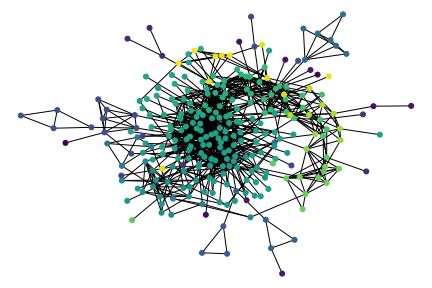
\includegraphics[width=\linewidth]{figures/saturated_graph.png}
\captionof{subfigure}{Saturated Graph}
\end{minipage}%
\hfill
\begin{minipage}{0.45\linewidth}
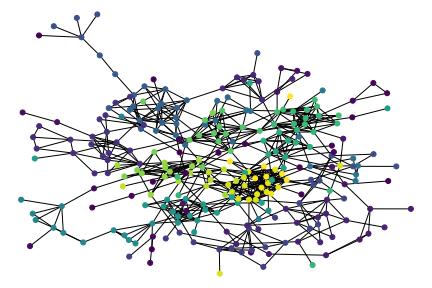
\includegraphics[width=\linewidth]{figures/fixed_graph.png}
\captionof{subfigure}{Fixed Graph}
\end{minipage}
\captionof{figure}{Generated graphs before and after addressing the saturation issue, 250 iterations each, colored by Apt-Markakis product}
\end{center}


We experimented with several ways of solving this, the most obvious being putting limits on the number of edges a node can have. While that did solve the issue, it had numerous flaws, the most obvious of which being it's contrived and not representative of anything in the real world, and it also prevented the graph from being scale-free, as no nodes could exceed an arbitrary limit in degree. The next thing we tried was logarithmically decreasing the $sim\_thresh$ value, which worked quite a bit better and resulted in better community differentiation, but again felt like a contrived method and not at all natural. \\

We eventually settled on a combination of fixes, and while they don't perfectly solve the problem, they do have the advantage of not involving arbitrary parameter changes or caps. We changed the Apt-Markakis sampling distribution to $Beta(0.75, 0.75)$  from $\mathcal{U}(0, 1)$, introduced a bucketing system for the Apt-Markakis diffusion process, and also introduced Gaussian noise each time a node adopts a product. We settled on these changes by noticing that in our Apt-Markakis step, node products tended to skew towards the middle, resulting in many nodes with similar products and thus vastly increasing the amount of nodes that can have edges added in the Schelling step. \\

The main change we made was the introduction of a bucket system for the product adoption. We do this by working probabilistically through dividing neighbor opinions into a histogram, and then sampling a new opinion from that histogram based on the amount of nodes falling into its buckets. This introduced a degree of randomness that seems to address the saturation issue, and combined with the Beta distribution increases the average clustering while maintaining a similar modularity. \\

The choice of the beta distribution stemmed from the same issue that drove the bucket system, the nodes products skewing towards the center. Before we implemented the bucket system, we experimented with using a beta distribution to sample products from, and noticed that while it seemed to help a bit, it still had the same skew problem. The $Beta(0.75, 0.75)$ distribution adopts a U shape that pushes weight towards the upper and lower ends of the range, meaning new nodes are more likely to have products closer to 0 or 1, and less likely to have products in the middle of that range. While this problem was better solved by using the bucketing system, we did notice that using the beta distribution and the bucket system together led to a higher average clustering of roughly 0.05 as well as a close to uniform distribution of the final products. Histograms of products with the various solutions can be seen in figure 3.2. \\

Unfortunately neither of these methods completely solved the issue, as the network still seems to saturate after more than a few thousand iterations. At only a few hundred iterations however, communities are very clearly separated as can be seen in figure 3.1. Saturation at larger amounts of iterations may well be a fundamental limit to the combination of models: at the very least no obvious solution presents itself beyond introducing still more models, which we hope to avoid. \\


\begin{center}
\begin{minipage}{0.45\linewidth}
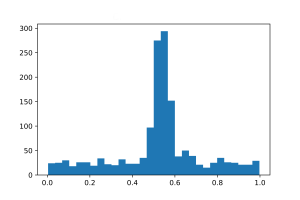
\includegraphics[width=\linewidth]{figures/hist.png}
\captionof{subfigure}{Model with Uniform Distribution}
\end{minipage}%
\hfill
\begin{minipage}{0.45\linewidth}
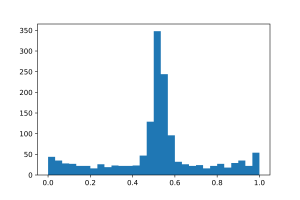
\includegraphics[width=\linewidth]{figures/hist3.png}
\captionof{subfigure}{Model with Beta Distribution}
\end{minipage}
\end{center}
\begin{center}
\begin{minipage}{0.45\linewidth}
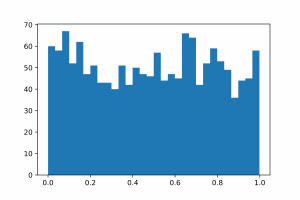
\includegraphics[width=\linewidth]{figures/hist4.png}
\captionof{subfigure}{Model with Buckets}
\end{minipage}
\hfill
\begin{minipage}{0.45\linewidth}
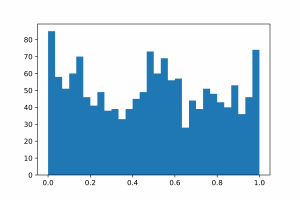
\includegraphics[width=\linewidth]{figures/hist2.png}
\captionof{subfigure}{Model with Buckets and Beta Distribution}
\end{minipage}
\captionof{figure}{Histograms of Apt-Markakis products}
\end{center}


\subsubsection{Time Complexity}

Part of the original plan was to have the Apt-Markakis products be vectors instead of scalars, but we quickly found that extending the model to the vector case was non-trivial, and in the implementations we tried time complexity soared for minimal changes in how the model evolved, and if anything increased the number of edges far more than the scalar model. \\

The obvious way to extend the Apt-Markakis model to vectors of products is to assume each index of the vector corresponds to a given category of product, and move on as normal. This effectively replicates the Apt-Markakis diffusion process $n$ times, where $n$ is the length of the vector. This is the method we implemented, where for each node with an unset product at index $i$ in its vector, the model checks if the neighbor threshold is met for its neighbors products at $i$. This then goes on to the Schelling step, where the similarity threshold becomes the L1 or L2 distance between the nodes Apt-Markakis vectors. \\

While this has the obvious effect of adding an additional scaling factor linear in the dimension of the Apt-Markakis vector length, but also increased the number of edges, as it seems this makes it harder for the Schelling thresholds to be met, which in turn increases model running time yet again. In all, the vector products seemed to hurt more than they helped both in terms of model quality and running time, and as such we settled on keeping the model scalar valued. \\

\section{Embedding System Design}

As with most neural networks, our embedding system is the result of much experimentation and trial and error. Our final autoencoder model makes use of a combination of a myriad of techniques, including Chebyshev convolutional layers, standard convolutions, batch normalization, noise layers, and more. We also augment input data with truncated random walks, and use reconstruction as well embedding losses. \\

\subsection{Random Walk Augmentation}

The input vector for a node $i$ in the network is initially just the $ith$ row of the adjacency matrix of the network. Drawing inspiration from DeepWalk \cite{perozzi2014deepwalk}, one of the more successful techniques we used was to augment that input with truncated random walks. Our method for this is simple enough: for each node in the graph we do a random walk with restart probability 0.1, and then treat all the nodes in the random walk as neighbors for the input. We redo the random walks at each training iteration, to both introduce noise and to get more information on context. We use a heuristic to determine walk length, $l = density * |V|$, as it seems to perform favorably compared to other methods. We define a restart probability of 0.1 to try to prevent the walks from getting too far away from their origin, a problem that becomes more pronounced the larger and denser the graphs are. \\

\subsection{Autoencoder Architecture}


\begin{center}

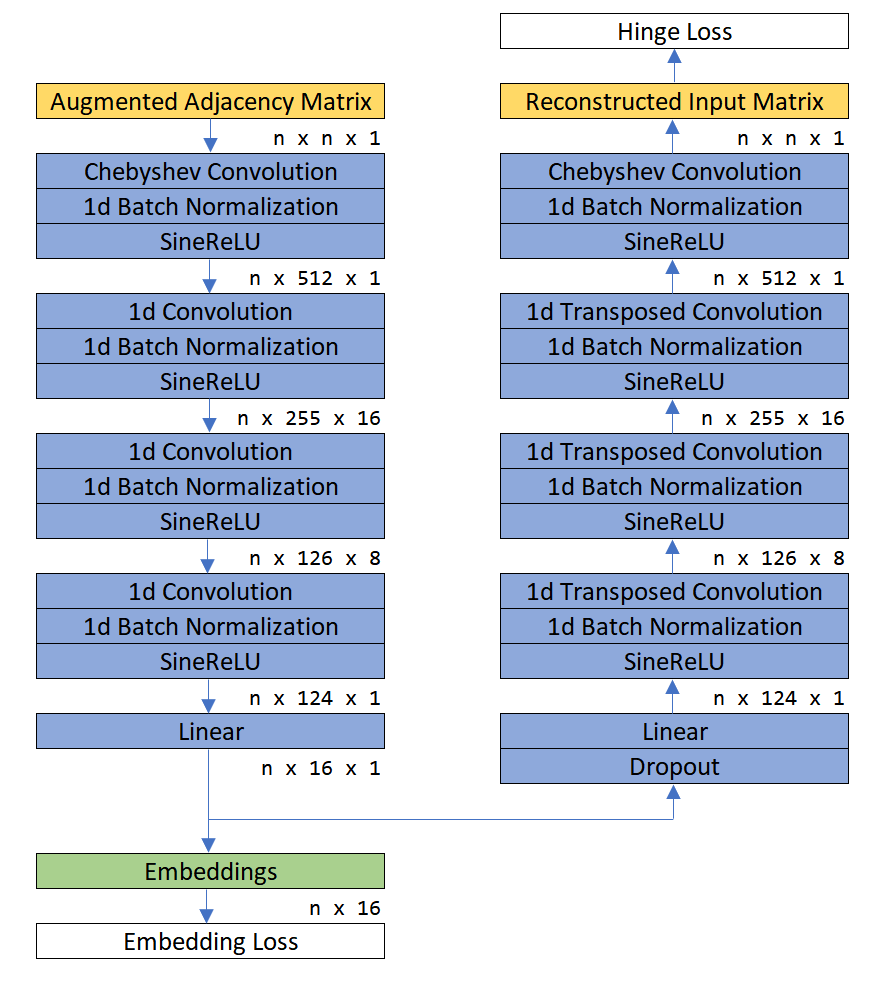
\includegraphics[width=\linewidth]{diagram/please.PNG}
\captionof{figure}{Architecture diagram of the autoencoder}
\end{center}


Our network is a standard convolutional autoencoder architecture, consisting of a Chebyshev convolutional layer, 3 standard convolutional layers, and a linear layer, interspersed with batch normalization layers and sineReLU activations on both the decoder and encoder sides, the only difference between the two being the decoder begins with a dropout layer. The network has two parameters: the mid layer size and hidden dimension size, set to 512 and 16 respectively in figure 3.3. \\

\subsection{Network Training}

Since our network is meant to work on dynamic networks, our training loop is nested, the outer looping over the networks from the first graph in the series to the last, and the inner being a standard training loop. We found that both Adam and SGD optimization with momentum worked well depending on dataset, and used two loss functions: a multi-class hinge loss for reconstruction error, and a cosine embedding loss to push adjacent nodes' embeddings closer together, and non-adjacent ones farther apart. \\

At each iteration of the outer loop, we load a new graph at the given time step and do some basic data processing. We then use a Net2WiderNet \cite{chen2015net2net} call on the input and output layers to accommodate any increase in the size of the graph.  In the inner loop, we re-run the random walk procedure to get a new augmented data matrix, and run negative sampling procedure to get input for the embedding loss, with positive examples being pushed closer together through hinge\_loss($x, y, 1$) and negatives apart through hinge\_loss($x, y, -1$). \\

\begin{algorithm}
\caption{Embedding System Training}
\begin{algorithmic}
\Function{train}{}
\For{$t$ in $time steps$}
\State load graph $G_{t}$
\If{$G_{t}.num\_nodes > G_{t-1}.num\_nodes$}
\State run Net2WiderNet on input and output layers
\EndIf
\State $X \gets$ random walk augmented adjacency matrix
\For{$epoch$ in $epochs$}
\State $recon, embeddings \gets model(X)$
\State $hinge \gets $ hinge\_loss($X, recon$)
\State $neighbors \gets$ [random\_neighbor($u, G_t$) for $u$ in $G_t$]
\State $cosine \gets$ cosine\_loss($embeddings, embeddings[neighbors], 1$)
\For{$\_$ in range(25)}
\State $negatives \gets$ [random\_node($G_t$) for $\_$ in $G_t$]
\State $cosine$ += cosine\_loss($embeddings, embeddings[negatives], -1$)
\EndFor
\State $loss = hinge + cosine$
\State backprop($loss$)
\EndFor
\EndFor
\EndFunction
\end{algorithmic}
\end{algorithm}

\subsection{Network Evaluation}

Our primary method of evaluating the quality of embeddings was using them for clustering problems. After embeddings were generated, we ran several K-means runs to cluster them, and then defined those clusters as partitions on the underlying graph and compared their modularity to that of the Louvain algorithm. We would have liked to reconstruct graphs from our embeddings to compare the reconstructed structure to the original, but unfortunately our choice of loss function as well as the augmented data prevented us from reconstructing graphs with any accuracy. Our reconstructions also prevented us from analyzing link prediction effectively, as the only method we could use was evaluating embedding proximity which provides no strong cutoffs for when there is or isn't a link. Another important metric we evaluated was embedding stability, a measure how much the embedding for a given node changed at any given time step, through simple checks of $||e_{i,t} - e_{i,t-1}||_2$, where $e_{i,t}$ is the embedding of node $i$ at time $t$, or alternatively but not equivalently $||E_{t} - E_{t-1}||^2_F$, where $E_t$ is the matrix of all embeddings at time $t$. \\

\subsection{Implementation}

Our autoencoder was implemented with NetworkX, PyTorch, and PyTorch Geometric, all of which were chosen due to our prior familiarity with them. We are largely happy with the results we were able to achieve, although we don't doubt there are better network architectures and training techniques waiting to be discovered, as our model was the result of much trial and error. \\

\subsubsection{Designing the Augmented Data Matrix}

In our initial plan, we planned to draw inspiration from artificial ant colony algorithms \cite{bertelle2006organization, zhou2015ant} through the use of pheremones on our graph that would be preserved at each time step. In normal artificial ant colony algorithms, ants function as walkers on the graph that leave a pheromone on each edge they traverse, and the more pheromones on an edge, the higher chance an ant will transition using it. We planned to do the opposite of this, with higher pheromone levels decreasing transition probability, so as to promote further exploration of the graph. This would have been especially useful in giving preference to new edges added at any given time step. \\

While we did see some improvements with the ant colony method, computation time soared as we had to compute transition probabilities at each step of each walker, as the pheromone levels were dynamic. While we believe this could be addressed with further optimization, the improvements to model results were small enough compared to the increase in running time that we did not pursue the method further. \\

\subsubsection{Designing the Network Architecture}

The network architecture went through several distinct phases of development. Early on we had difficulty installing PyTorch Geometric and attempted to create a fully linear network, but as one would expect training times were high and results were poor. In the next iteration we attempted a fully graph-convolutional network, and as part of that experimented with numerous types of graph convolution layers. Lastly, we found that a combination of graph convolutions and standard convolutions seemed to work best, and settled on that structure. \\

One unfortunate limitation we ran into in testing was the inconsistent implementation of convolutional layers in PyTorch Geometric. While this wouldn't normally be an issue, we were using custom Net2Net calls on the input and output layers, which were always graph convolutional layers. These inconsistencies resulted in us needing to rewrite the Net2Net each time we tried a new layer, and as such we weren't able to test as many as we would have liked. That being said, we did try out several methods including  Morris et al's $k$-GNN \cite{morris2019weisfeiler} and Kipf et al's GCN \cite{kipf2016semi}, and while they did tend to be faster, they also generated notably lower quality embeddings. \\

One unusual choice we made in our architecture was the use of the SineReLU activation function. 

\[ SineReLU(x) =  \begin{cases} 
          0.025(sin(x) - cos(x)) & x < 0 \\
          x & x\geq 0
       \end{cases} \]
       
SineReLU has the advantage of always being differentiable, and the below zero component is best understood as being a noisy gradient to promote further exploration. We did notice a marginal increase in performance with this function, and while it's quite possible that itself is just noise we decided to keep it anyways. \\

\subsubsection{Designing the Loss Functions}

We initially used simple L1 and L2 loss for our reconstruction error, but quickly found that the model would just learn the degree of a node divided by the total number of nodes, a classic case of learning the average. We addressed this by making the problem a classification problem instead of a direct reconstruction, as in that context the output becomes binary: either a given node is a neighbor or it isn't. While this does have the effect of making it difficult to impossible to reconstruct a graph directly from the embeddings, performance was vastly improved and we feel that is a small price to pay. PyTorch provides two easy loss functions for the multi-label classification case: binary cross entropy and hinge loss. The latter seemed to both converge faster, and yield better embeddings in general, so we stuck with the hinge loss in our final model. \\

The other loss function we used was a cosine embedding loss to influence how close the embeddings are to each other. This is a standard technique in embedding contexts where we know pairwise which data points should be close together and which farther apart. The obvious route to take, and the one we used, is that two nodes should be embedded close together if they are neighbors, and farther apart if they are not. This was easy enough to do, and we followed a standard negative sampling heuristic of using 25 negative examples for each positive, in our case 25 non-neighbors and 1 neighbor at each iteration of the model. Increasing the number much beyond this would slow down the model more than we would like, and decreasing it tended to marginally decrease embedding quality. \\

\subsubsection{Modularity and Shortest Paths}

Another area we experimented in was encoding extra information into our embeddings so as to better represent the network's structure, specifically optimizing modularity of the resulting embeddings, and encoding shortest path length between two nodes. Both these methods increased computation time and decreased embedding quality, so they were ultimately abandoned despite efforts to fix them. \\

In encoding modularity, we attempted to force our embeddings to be linearlly reducable to assignment vectors so as to be optimized against a modularity matrix, as done by Newman \cite{newman2006modularity}, and in a deep learning context by Yang et al \cite{yang2016modularity}. Unfortunately in the vain of Brandes et al \cite{brandes2006maximizing} we rapidly ran into several issues. The first being the optimization space appeared extremely non-convex and it was difficult to converge to any solution, much less a good one. The other was it was difficult to constrain our assignment vectors such that they summed to one without increasing the depth of the layer translating the embeddings to assignments, which then had the effect of decorrelating the two entirely. Fixing any given issue seemed to lead to raising others, and in the end even the assignment vectors didn't get good modularity, and we decided to move on without pursuing it further. \\

We had more success in encoding shortest path distances, following the methods of Rizi et al \cite{rizi2018shortest}. For each node in the graph, we randomly choose another and compute their shortest path length, and then have a new layer of the network translate the average of their two embeddings into a shortest path length. While we were able to approximate the path lengths very well, it did not increase embedding quality by any metric, and as such we abandoned that method as well. \\

\subsubsection{Visualizing the Embeddings}

While loss metrics are useful in understanding how well the embeddings represent the data, it is almost always useful to inspect the results visually as well to check for issues that the loss might not capture. The obvious way to do this is to make the hidden dimension 2 so it can be plotted directly, or to introduce another layer to encode the embeddings down to 2 values as well. While the latter method has merit, since our data tended to be highly clustered we decided to use TSNE \cite{maaten2008visualizing}, a dimensionality reduction technique that prioritizes preserving community structure in the original space. \\

Standard implementations of TSNE work fine for visualizing the embeddings at a given time step, but we quickly ran into issues with consistency across multiple time steps. TSNE does not in its normal form support online updating, although workarounds have been proposed \cite{van2009learning}. We overcame this issue by simply initializing the TSNE weights at time $t$ to the ones learned step $t-1$, and initialized any new nodes to $\mathcal{N}(\mu(E_{t-1}), I)$. While this led to more unstable visualizations than we would have liked, it was easy to implement and was still a significant step up from retraining from scratch each time. \\

%%%%%%%%%%%%%%%%%%%%%%%%%%%%%%%%%%%%
\chapter{Results}

We were generally satisfied with the results of both our network model and embedding system, although both did have shortcomings that we feel are inevitable in trying to capture real-world phenomena. Our network model ended up being a jack of all trades, master of none, which was to be expected in combining models as we did. Our embedding system does seem to consistently meet DynGEM's performance when restricted in running time, and beat it when it is allowed to run longer, especially on networks with more complex  topologies. \\ 

\section{The Network Model}

Our goal in designing the network model was for it to be able to create synthetic, dynamic graphs that are similar to real-world data. In this, we believe we were successful by most metrics. The degree distributions of our networks only followed a power-law in their upper tails, there was no discernible increase in diameter with network size but average path lengths and clustering were consistent with small-world behavior, and they seemed to be length-scale invariant but only up to a few renormalizations. \\

\subsection{Scale-Freeness}

While our resulting networks were not strongly scale-free throughout, they were weakly so in the same manner as most real-world social networks, in that they are scale free for large values around the upper tail. The degree distributions of our model as well as a Facebook dataset and a run of the Barabási–Albert model can be seen in figure 4.1. \\


\begin{center}
\begin{minipage}{0.45\linewidth}
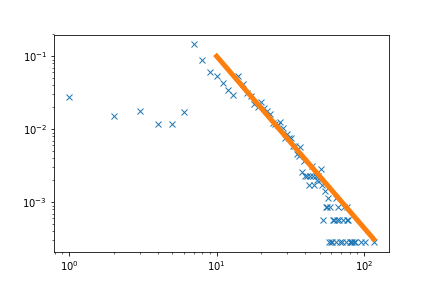
\includegraphics[width=\linewidth]{figures/degs/1.png}
\captionof{subfigure}{2500 Model Iterations, $\gamma \approx$ 2.35}
\end{minipage}%
\hfill
\begin{minipage}{0.45\linewidth}
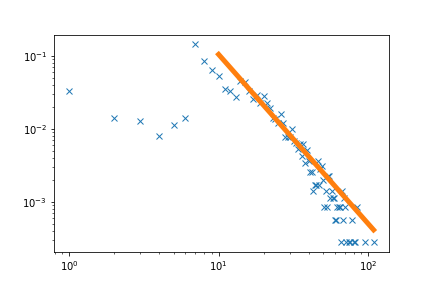
\includegraphics[width=\linewidth]{figures/degs/3.png}
\captionof{subfigure}{2500 Model Iterations, $\gamma \approx$ 2.31}
\end{minipage}
\end{center}
\begin{center}
\begin{minipage}{0.45\linewidth}
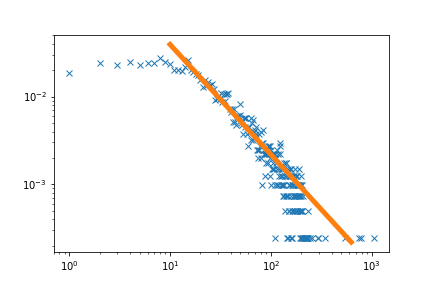
\includegraphics[width=\linewidth]{figures/degs/facebook.png}
\captionof{subfigure}{SNAP's Facebook Dataset, $\gamma \approx$ 1.25}
\end{minipage}
\hfill
\begin{minipage}{0.45\linewidth}
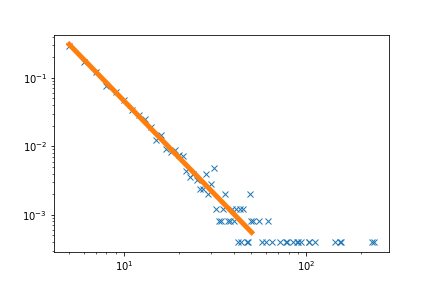
\includegraphics[width=\linewidth]{figures/degs/ba.png}
\captionof{subfigure}{Barabási–Albert Model, $\gamma \approx$ 2.74}
\end{minipage}
\captionof{figure}{Degree Plots and Power Law Fits of Graphs}
\end{center}

We believe that the non-power law lower tail stems from the Schelling step, as in the course of model execution most nodes either become unhappy and move, or some other node moves into their neighborhood, this increasing the degree above what we'd see in a truly scale-free network. Regardless, ignoring the non-power law lower tail is common in determining whether a network is scale-free \cite{broido2019scale}, and for the upper tail the fit is good and $\gamma$ seems strongly within the $(2,3)$ range. \\

\subsection{Small-Worldedness}

We identified two metrics to test small-worldedness with: a combination of average clustering and shortest path length compared to random graphs, and the growth in diameter over time. We are very satisfied in the former showing small-world characteristics, but in the latter our model appears to work in a densification regime rather than the expected slow increase. \\

\subsubsection{Average Clustering and Path Length}

We found that over time, the average shortest path length $l_G$ converged to around 3.9, and that the average clustering coefficient $\bar{C}$ converged to around 0.17, both of which comfortably similar to what we'd expect, as Erdős–Rényi networks of comparable size have values of around 3 and 0.005, respectively. Although the average clustering coefficient is somewhat low, the data clearly indicates that the network has small-world properties, albeit weaker than we would like. The hard numbers can be found in table 4.1, and a visualization of $\bar{C}$ and $l_G$ for several runs of our model can be seen in figure 4.2. \\

\begin{center}
\begin{tabular}{l*{6}{c}r}
Model              & $|V|$ & $|E|$ & $l_G$ & $\bar{C}$ \\
\hline
Erdős–Rényi    & 3500 & 30545 & 3.135 & 0.005  \\
Synthetic      & 3525 & 27410 & 3.899 & 0.171  \\
Watts-Strogatz & 3500 & 28000 & 3.943 & 0.431  \\
\end{tabular}
\captionof{table}{Average clustering coefficients and shortest path lengths} 
\end{center}


\begin{center}
\begin{minipage}{0.45\linewidth}
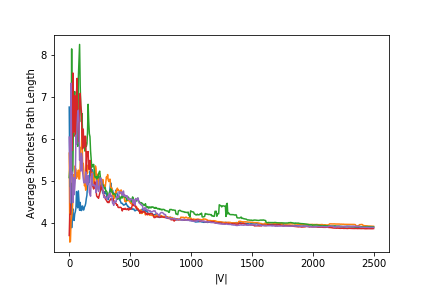
\includegraphics[width=\linewidth]{figures/lens.png}
\captionof{subfigure}{Average Clustering Coefficient}
\end{minipage}%
\hfill
\begin{minipage}{0.45\linewidth}
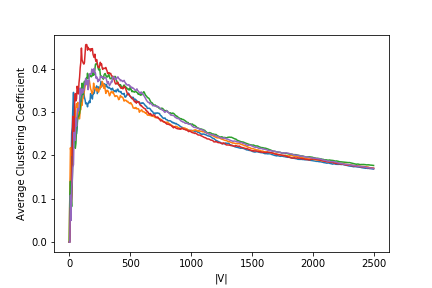
\includegraphics[width=\linewidth]{figures/clusts.png}
\captionof{subfigure}{Average Shortest Path Length}
\end{minipage}
\captionof{figure}{Metrics over time for 5 runs of the model}
\end{center}

\subsubsection{Diameter Dynamics}

An unexpected result we found in our model was that the effective diameters seemed to converge to around 5 rather than increase logarithmically as is expected in small-worlds. This fortunately has a straightforward cause, while the number of nodes increases only linearly in time, the increase in edges appears to follow a power law. This is an especially interesting result as this is near exactly what is described by Leskovec \cite{leskovec2007graph}, with the plot of number of nodes against number of edges following a power law with $a = 1.253$, similar to Leskovec's findings of a recommender system dataset. Figure 4.3.a shows the edge vs node growth power law, and figure 4.3.b shows the decreasing diameter over time for 5 model runs.  \\


\begin{center}
\begin{minipage}{0.45\linewidth}
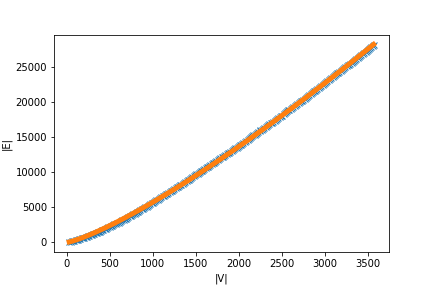
\includegraphics[width=\linewidth]{figures/densification.png}
\captionof{subfigure}{Densification regime, $a=1.253$}
\end{minipage}%
\hfill
\begin{minipage}{0.45\linewidth}
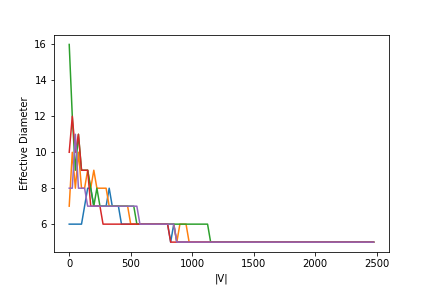
\includegraphics[width=\linewidth]{figures/diameters.png}
\captionof{subfigure}{Effective diameter over time}
\end{minipage}
\captionof{figure}{Densification metrics on 5 runs of the model}
\end{center}

We view this as a confirmation of the model's relation to the real-world: this is an emergent phenomena that we did not design for, or in fact even know the existence of beforehand that nonetheless exists in our networks despite the fact that edge creation and deletion is purely governed by the Schelling process. \\

\subsection{Self-Similarity}

Another unexpected result we found was self-similarity, although as with small-worldness our model appears only weakly self-similar. Self-similarity is the least well-defined metric we evaluated, and as such there were several paradigms to consider. The first method we examine determines self-similarity by measuring characteristics of the Girvan-Newman community detection algorithm \cite{guimera2002self}, and the second uses a more standard box counting and renormalization approach \cite{song2007calculate}. \\

\subsubsection{Girvan-Newman Self-Similarity}

Guimera et al \cite{guimera2002self} draw inspiration from river and drainage basin literature and evaluate 3 main features of the Girvan-Newman communities: The structure of its dendrogram, the cumulative probability distribution of its community sizes, and lastly the Horton-Strahler numbers. We compare our model to an Erdős–Rényi graph, the fractal model proposed by Song \cite{song2006origins}, and Guimera's email dataset. \\

Dendrograms of the GN algorithm on random graphs tend to be straight lines, but running the algorithm on our model after 1250 iterations leads to a similar structure as Guimera's email dataset. This is the most subjective measurement as we only inspect the graphs visually. A cursory glance at the GN dendrograms in figure 4.4 confirms the similarity to the email dataset as well as such natural structures as Brownian trees. \\


\begin{center}
\begin{minipage}{0.45\linewidth}
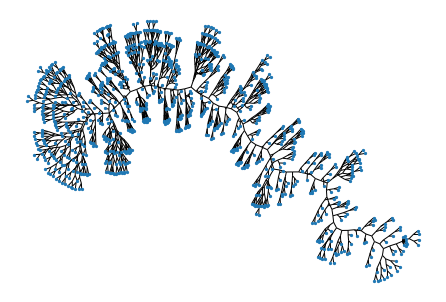
\includegraphics[width=\linewidth]{figures/er_dendro.png}
\captionof{subfigure}{Erdős–Rényi graph, $|V| = 1000$}
\end{minipage}%
\hfill
\begin{minipage}{0.45\linewidth}
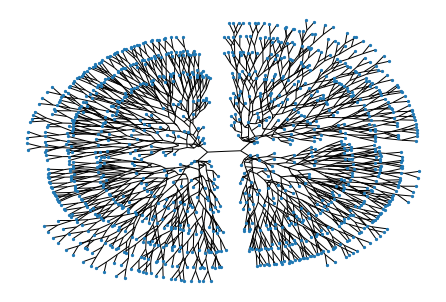
\includegraphics[width=\linewidth]{figures/fractal_dendro.png}
\captionof{subfigure}{Song fractal model, $|V| = 1038$}
\end{minipage}%
\hfill
\begin{minipage}{0.45\linewidth}
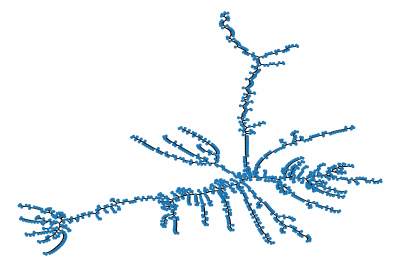
\includegraphics[width=\linewidth]{figures/uvl_dendro.png}
\captionof{subfigure}{Guimera's email dataset, $|V| = 1133$}
\end{minipage}%
\hfill
\begin{minipage}{0.45\linewidth}
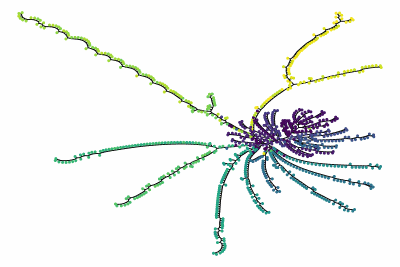
\includegraphics[width=\linewidth]{figures/1500_dendro.png}
\captionof{subfigure}{Synthetic model, $|V| = 913$, colored by Apt-Markis product }
\end{minipage}
\captionof{figure}{GN community dendrograms}
\end{center} 

\vspace{1pt}


We can expand our analysis of the communities by examining the cumulative community size distribution, and again can see obvious similarities to real-world phenomena as well as Guimera's data in figure 4.5. The power law is a noticeably worse fit for the same lower tail of our data however, with a significantly lower $R^2$ and visually it seems another distribution might be a better fit. Regardless, the basic structure of the curves seems similar enough to warrant further investigation. \\


\begin{center}
\begin{minipage}{0.45\linewidth}
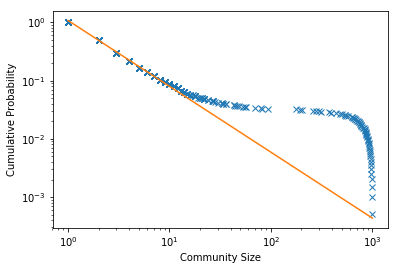
\includegraphics[width=\linewidth]{figures/er_curve.png}
\captionof{subfigure}{Erdős–Rényi graph, exponent $\approx 1.1$, , $R^2 = 0.99$}
\end{minipage}%
\hfill
\begin{minipage}{0.45\linewidth}
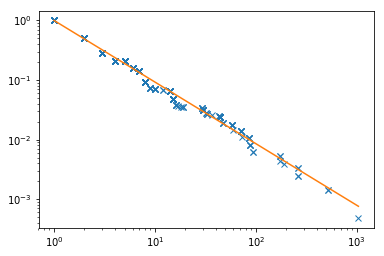
\includegraphics[width=\linewidth]{figures/fractal_curve.png}
\captionof{subfigure}{Song fractal model, exponent $\approx 1.0$, , $R^2 = 0.99$}
\end{minipage}%
\hfill
\begin{minipage}{0.45\linewidth}
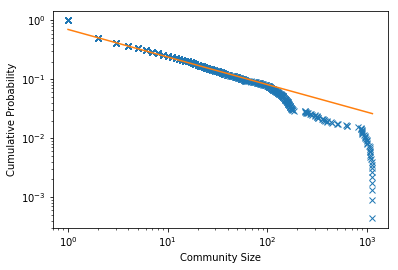
\includegraphics[width=\linewidth]{figures/uvl_curve.png}
\captionof{subfigure}{Guimera's email dataset, exponent $\approx 0.48$, $R^2 = 0.99$}
\end{minipage}%
\hfill
\begin{minipage}{0.45\linewidth}
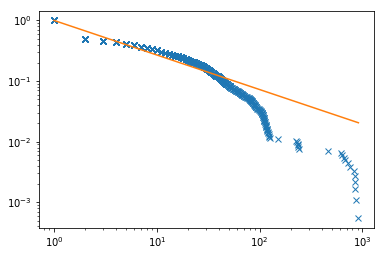
\includegraphics[width=\linewidth]{figures/1750_curve.png}
\captionof{subfigure}{Synthetic model, exponent $\approx 0.57$, $R^2 = 0.83$ }
\end{minipage}
\end{center}
\captionof{figure}{GN cumulative community distributions}


The last metric they evaluate involves the Horton-Strahler numbers \cite{horton1945erosional, strahler1952dynamic}, which were initially developed to describe the size of tributaries and rivers in networks. A low number means there is small upstream flow, and a high number indicates a large amount of upstream flow. In our case, flow corresponds to community structure, where a higher number corresponds to higher community structure upstream of a given node. \\


\begin{center}
\begin{minipage}{0.45\linewidth}
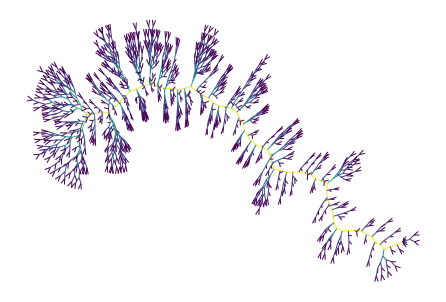
\includegraphics[width=\linewidth]{figures/er_bifurcations.png}
\captionof{subfigure}{Erdős–Rényi graph, $max(HS) = 7$}
\end{minipage}%
\hfill
\begin{minipage}{0.45\linewidth}
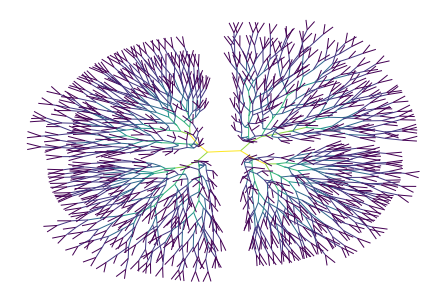
\includegraphics[width=\linewidth]{figures/fractal_bifurcation.png}
\captionof{subfigure}{Song fractal model, $max(HS) = 8$}
\end{minipage}%
\hfill
\begin{minipage}{0.45\linewidth}
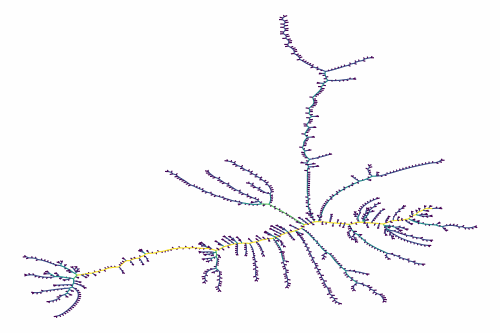
\includegraphics[width=\linewidth]{figures/uvl_bifurcations.png}
\captionof{subfigure}{Guimera's email dataset, $max(HS) = 5$}
\end{minipage}%
\hfill
\begin{minipage}{0.45\linewidth}
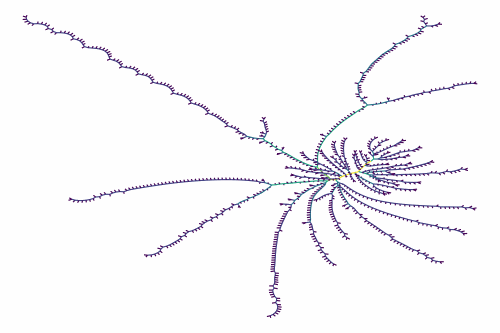
\includegraphics[width=\linewidth]{figures/1750_bifurcations.png}
\captionof{subfigure}{Synthetic model, $max(HS) = 6$ }
\end{minipage}
\captionof{figure}{HS indices}
\end{center}


Examining the HS indices in and of themselves as in figure 4.6 doesn't yield a great deal of information, but they can be used to calculate a useful metric of self-similarity: bifurcation ratios. The bifurcation ratio is defined for $1 < i < max(HS)$ for a given graph, and is simply $B_i = n_i / n_{i+1}$, where $n_i$ is the number of branches with HS index $i$. When $\forall i B \approx B_i$, the network is said to be self-similar, as when the ratios are all similar that means that each branch's subtrees have a similar structure. We can evaluate in this by simply inspecting the mean and standard deviation of all $B_i$ values, which yields some interesting results, shown in table 4.2. \\

\begin{center}
\begin{tabular}{l*{6}{c}r}
Model              & $|V|$ & $|E|$ & $\mu$ & $\sigma$ \\
\hline
Erdős–Rényi    & 1000 & 2461 & 3.385 & 1.332  \\
Song Fractal   & 1038 & 1296 & 2.761 & 0.594  \\
Guimera Emails & 1133 & 5452 & 5.872 & 0.889  \\
Synthetic      & 913  & 4992 & 4.869 & 3.772  \\
\end{tabular}
\captionof{table}{Mean and Standard Deviation of $B$ for several models}
\end{center}

Obviously the standard deviation on our model is significantly higher than the rest. When examining the $B_i$ values directly in table 4.3, we notice that $B_1$ is a major outlier, and removing it yields $\mu = 3.002$ and $\sigma = 0.592$. Unfortunately we have no explanation as to why our network has so many branches with $HS = 1$ compared to the other models, and as such we refrain from making strong conclusions with this method. \\

\begin{center}
\begin{tabular}{l*{6}{c}r}
Model              & $B_1$ & $B_2$ & $B_3$ & $B_4$ & $B_5$ & $B_6$ & $B_7$ \\
\hline
Erdős–Rényi      & 2.6  & 2.6 & 3.1 & 4.1 & 6.0 & 2.0 & -  \\
Song Fractal      & 2.4  & 3.1 & 2.1 & 3.8 & 3.0 & 3.0 & 2.0  \\
Guimera Emails      & 6.3  & 5.7 & 4.6 & 7.0 & - & - & -  \\
Synthetic      & 12.3  & 3.4 & 3.1 & 3.5 & 2.0 & - & -  \\
\end{tabular}
\captionof{table}{$B$ values for several models}
\end{center}

\subsubsection{Box Counting Self-Similarity}

A second method of evaluating self-similarity more rooted in geometry is proposed by Song et al \cite{song2005self}, relying on box counting. In the geometric domain, this involves iteratively tiling a shape with smaller and smaller boxes, at each time evaluating how many boxes bound some part of the shape. This of course doesn't trivially generalize to networks, but Song proposes to define boxes as neighborhood graphs whose radius corresponds to box size. Nodes in the graph are randomly sampled and box with nodes in their neighborhood until the entire graph is covered. \\

Song proposes two new metrics to evaluate self-similarity: the fractal dimension $d_B$, which is the exponent in the power law relation between box size and number of boxes needed to cover the network, and $d_k$, which relates to how stable a network is to renormalization. Our model seems to again be weakly self-similar under these metrics the $d_B$ metric shown in figure 4.7, but it was difficult to calculate $d_k$ given the relatively small size of our networks: Song calculated his against the entire http-level  Internet. \\


\begin{center}
\begin{minipage}{0.45\linewidth}
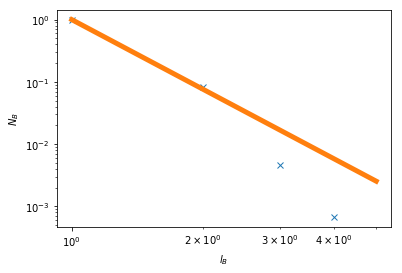
\includegraphics[width=\linewidth]{figures/ba_hausdorff.png}
\captionof{subfigure}{Barabási–Albert graph, $d_B = 3.71$}
\end{minipage}%
\hfill
\begin{minipage}{0.45\linewidth}
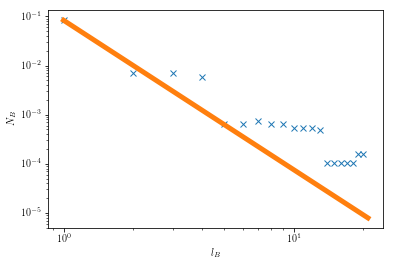
\includegraphics[width=\linewidth]{figures/song_hausdorff.png}
\captionof{subfigure}{Song fractal model, $d_B = 3.04$}
\end{minipage}%
\hfill
\begin{minipage}{0.45\linewidth}
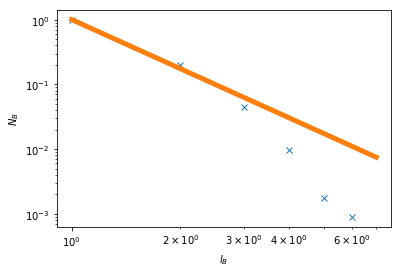
\includegraphics[width=\linewidth]{figures/uvl_hausdorff.png}
\captionof{subfigure}{Guimera's email dataset, $d_B = 2.52$}
\end{minipage}%
\hfill
\begin{minipage}{0.45\linewidth}
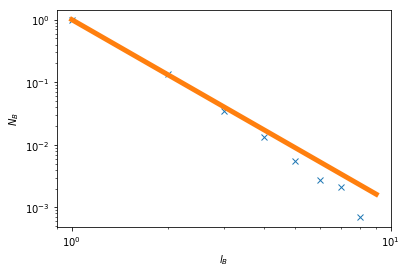
\includegraphics[width=\linewidth]{figures/1500_hausdorff.png}
\captionof{subfigure}{Synthetic model, $d_B = 2.94$ }
\end{minipage}
\captionof{figure}{Neighborhood radius against number of nodes needed to cover the networks}
\end{center}


The main thing to notice here is how Song's fractal model skews above the fitted curve, a behavior Song also finds in his plot of the Internet. All other models seem to skew below the plot, although they all are well described by a power law. Based off the loose findings from the GN method as well as the fact that our model is closer to the power law curve than Guimera's emails dataset, we do conclude that our model is weakly self-similar. \\

Unfortunately in both methods evaluating self-similarity requires very large datasets to allow for examination at numerous scales, something we just were not able to both run our model for, and use the requisite algorithms on. Nonetheless, our basic findings do indicate that our networks are self-similar to some degree, and further examination could be a useful research direction. \\


\subsection{Modularity}

The networks generated by our model tended to be highly modular. This is clear for visual inspections of small networks of a few hundred nodes shown in figure 4.8, but as the networks grow we needed a new metric to verify that modularity was maintained. We accomplished this by using the Louvain algorithm \cite{blondel2008fast} to detect communities and then check the modularity $Q$ of those communities, shown in table 4.4. \\


\begin{center}
\begin{minipage}{0.45\linewidth}
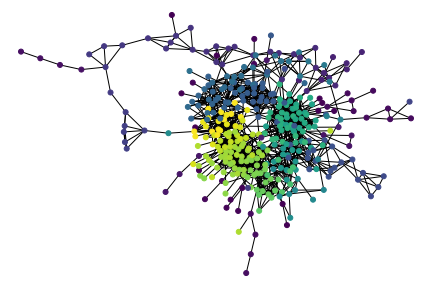
\includegraphics[width=\linewidth]{figures/1.png}
\end{minipage}%
\hfill
\begin{minipage}{0.45\linewidth}
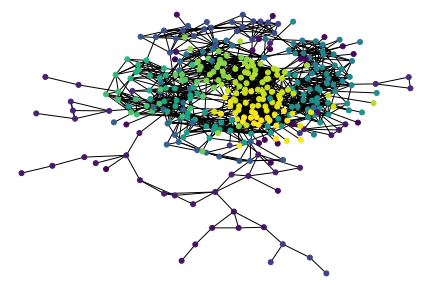
\includegraphics[width=\linewidth]{figures/3.png}
\end{minipage}
\captionof{figure}{Two generated graphs after 350 iterations colored by Apt-Markakis product}
\end{center}


\begin{center}
\begin{tabular}{l*{5}{c}r}
              & $V$ & $E$ & $Q$ \\
\hline
Erdős–Rényi & 3500 & 24503 & 0.224 \\
Watts-Strogatz & 3500 & 2800 & 0.792 \\
Song Fractal & 3512 & 4096 & 0.926 \\
Guimera Emails & 1133 & 5452 & 0.570 \\
CORA & 5278 & 5278 & 0.813 \\
Synthetic & 3525 & 27410 & 0.714 \\
\end{tabular}
\captionof{table}{Modularity of several models}
\end{center} 

The modularity scores on our network were the second highest of the models and datasets, below only CORA, and the Song Fractal and Watts-Strogatz models. Fractal networks in general are highly modular almost by definition, explaining the strong modularity of the Song networks. Our model scored close to Watts-Strogatz and CORA but was not quite comparable, which we attribute to the edge saturation issue that we were unable to completely solve: it's likely that several of the edges are superfluous even for maintaining Schelling stability. \\

\section{The Embedding System}

Our embedding system was able to consistently outperform DynGEM \cite{goyal2018dyngem}, the only other dynamic growing embedding model that had reference code we could find. Although several other models have been proposed \cite{ma2018dynamic, trivedi2018representation}, we were unable to find reference implementations and as such restrict ourselves to DynGEM. We compare our embeddings to DynGEM as well as Node2Vec \cite{grover2016node2vec} representations learned separately on each graph and show large improvements in both clustering and stability on both synthetic and real-world data. We found that Adam and SGD optimizers seem to perform well in general but on some datasets one is significantly better than the other: unless otherwise specified performances listed were trained using SGD. \\

\subsection{CORA Sanity Check}

Before checking our models's performance on other metrics, we wanted to test that it was learning useful embeddings at all on a real-world dataset. We used the CORA dataset \cite{sen2008collective} for this, as it is a standard dataset for classification with ground truth labels. While the dataset is unfortunately not dynamic, it is a standard benchmark for node embedding systems and as such we view it as a natural choice for a simple sanity check. For our check, we convert it to an undirected graph and take only the giant component. \\

We checked network performance on it by generating embeddings and then clustering with k-means. We then match these clusters to the ground truth values and took the best of 10 performances to get an accuracy score that we compare the models on. Importantly, we do not consider any data other than adjacency information in generating the embeddings for any of our systems, as we wanted to make our system as generalizable as possible. Figure 4.9 show our model trained with Adam significantly outperforming Node2Vec and DynGEM in this metric, and as such we conclude our system is working as expected. \\


\begin{center}
\begin{minipage}{0.45\linewidth}
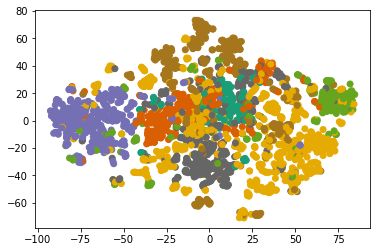
\includegraphics[width=\linewidth]{figures/cora/node2vec_true.png}
\captionof{subfigure}{Node2Vec, $acc = 0.599$}
\end{minipage}
\hfill
\begin{minipage}{0.45\linewidth}
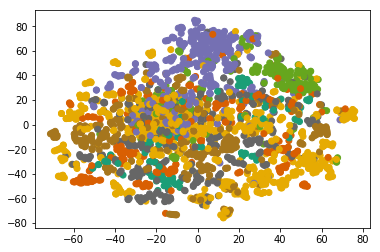
\includegraphics[width=\linewidth]{figures/cora/dyngem_true.png}
\captionof{subfigure}{DynGEM, $acc = 0.425$}
\end{minipage}%
\hfill
\begin{minipage}{0.45\linewidth}
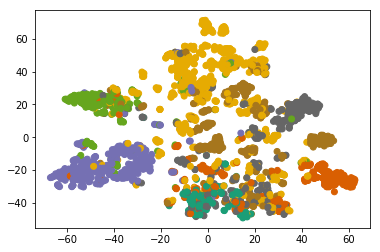
\includegraphics[width=\linewidth]{figures/cora/true_our_model.png}
\captionof{subfigure}{Our System, $acc = 0.692$}
\end{minipage}%
\captionof{figure}{CORA performance by model, colored by paper classification}
\end{center}


\subsection{Clustering Performance}

The area we saw the largest improvement over existing encoding methods was clustering performance. When trained for either the same amount of running time or epochs, our model significantly outperforms DynGEM and Node2Vec on our synthetic dataset but faces more issues with the AS \cite{leskovec2005graphs} and Irvine \cite{panzarasa2009patterns} datasets. \\

We evaluate clustering performance by first running the Louvain algorithm to get a reference performance as well as an upper bound on the number of communities to check $n$. We define the best clustering performance as the maximum modularity among k-means clustering run 5 times each for $num\_clusters \in (2, n)$. We then compare the models using the average performance over all embeddings at all time steps. Table 4.5 contains clustering performances from the three algorithms on the three datasets. The graphs from the synthetic model correspond to a single run at 10 step intervals between 2500 and 2600, and the AS data is a subset of the first 10 graphs separated by 5 steps each. The Irvine dataset is the giant component over 10 snapshots corresponding to 10 percentiles of the timestamps.  \\

\begin{center}
\begin{tabular}{l*{5}{c}r}
              & Node2Vec & DynGEM & Our System & $Louvain$ \\
\hline
Synthetic Data    & 0.68 & 0.66 & \textbf{0.72} & $0.76$  \\
AS Dataset   & \textbf{0.29} & 0.13 & 0.17 & $0.65$  \\
Irvine Dataset   & \textbf{0.33} & 0.00 & 0.27 & $0.34$  \\
\end{tabular}
\captionof{table}{K-means clustering performance of embeddings}
\end{center} 

Our model likely runs into issues on the AS dataset because of the removal of nodes at some time steps, something that we did not plan for and does not happen in our synthetic model. This throws off training as we keep the removed nodes as isolates, which appears to impede training on the embedding loss of both it and the remaining nodes. DynGEM exhibits the same issue but significantly more so, and although Node2Vec does beat our performance, our embeddings are much more stable. The Irvine dataset has a low clustering coefficient and the Louvain algorithm struggles to find modular communities, which appears to be a real issue for DynGEM and to a lesser extent our system. \\

\subsection{Embedding Stability}

While our model was unable to beat Node2Vec on clustering performance, we were able to outperform both it and DynGEM on stability, which with inspiration from DynGEM we define as

\[ \text{stability} = \frac{|| E_t - E_{t-1}||^2_F}{||A_t - A_{t-1}||^2_F} \]
 
where $E_t$ is the embedding matrix and $A_t$ is the adjacency matrix both at time $t$. We used the same generated embeddings and graphs as in modularity testing, and results are shown in table 4.6. \\

\begin{center}
\begin{tabular}{l*{5}{c}r}
              & Node2Vec & DynGEM & Our System \\
\hline
Synthetic Data    & 20.52 & 58.53 & \textbf{4.35}  \\
AS Dataset   & 4.01 & 2.68 & \textbf{0.56}  \\
Irvine Dataset   & 9.01 & 22.98 & \textbf{2.87}  \\
\end{tabular}
\captionof{table}{Embedding stability under Frobenius norm}
\end{center} 

One notable issue is that DynGEM seems to do worse than even Node2Vec on our synthetic model and the  Irvine dataset, which we think is attributable to overfitting. We can run DynGEM for fewer iterations and get more stable embeddings than Node2Vec, although also causing significant degradation to clustering performance. Regardless, the results indicate that our embeddings are more stable than DynGEM's as well as Node2Vec, highlighting the improvements gained by graph convolutions. \\

\subsection{Running Time}

Running time was difficult to evaluate with our model as we had to decide arbitrary stopping criteria based off when the model had converged, which was a time-consuming process in and of itself. We settled on using the running times of the model runs we used in analyzing stability and clustering performance as they should be representative of our model performance in general. \\

Table 4.8 shows the runtimes of the three models. We found that Node2Vec and DynGEM tended to converge faster than our model on smaller networks, but our system began to outperform them as network size increased. Both models did significantly improve over Node2Vec's training time for the larger networks however, as shown in the chart below. We attribute this largely to overhead complexity which is negligible in Node2Vec and DynGem, but for our model is linear in the number of nodes for constructing the augmented input matrix. \\

\begin{center}
\begin{tabular}{l*{5}{c}r}
              & Node2Vec & DynGEM & Our System \\
\hline
Synthetic Data    & 197 & \textbf{74} & 103  \\
AS Dataset   & 321 & 251 & \textbf{197}  \\
Irvine Dataset   & \textbf{52} & 138 & 103  \\
\end{tabular}
\captionof{table}{Embedding system running time}
\end{center} 

\subsection{Applications}

Our embedding system has many possible applications, ranging from the clustering discussed above to link prediction among many others. Two applications that fit naturally into our system and model however are anomaly detection and trajectory visualization. Anomaly detection is simple in our case, we merely need to show that our embeddings at a time step where an anomaly happens are significantly different than those at the step before. Trajectory visualization is another interesting thing, as it lets us see how a node moves in the embedding space when it is chosen as part of the Schelling step. \\

\begin{center}
\begin{minipage}{0.45\linewidth}
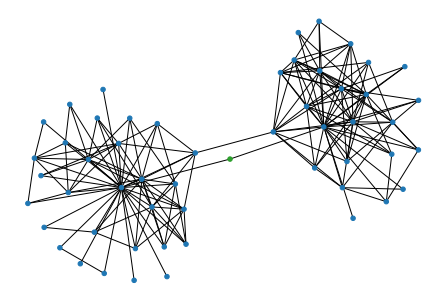
\includegraphics[width=\linewidth]{figures/tsne_graph1.png}
\captionof{subfigure}{Neighborhood of target at $t-1$}
\end{minipage}%
\hfill
\begin{minipage}{0.45\linewidth}
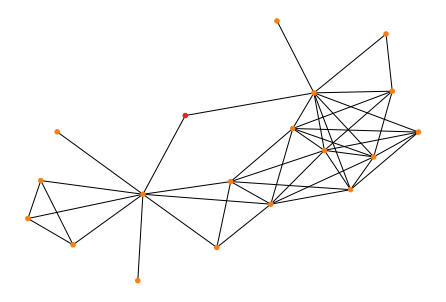
\includegraphics[width=\linewidth]{figures/tsne_graph2.png}
\captionof{subfigure}{Neighborhood of target at $t$}
\end{minipage}
\hfill
\begin{minipage}{0.45\linewidth}
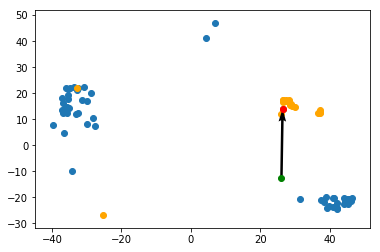
\includegraphics[width=\linewidth]{figures/tsne_trajectory2.png}
\captionof{subfigure}{Embedding space change}
\end{minipage}
\hfill
\begin{minipage}{0.45\linewidth}
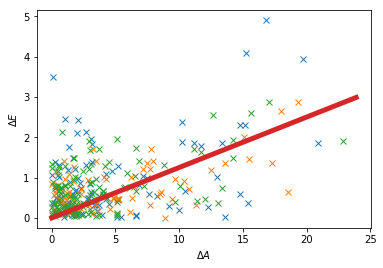
\includegraphics[width=\linewidth]{figures/emb_change.png}
\captionof{subfigure}{Embedding vs adjacency stability over three runs}
\end{minipage}%
\captionof{figure}{TSNE visualization of a Schelling step}
\end{center}

\subsubsection{Visualizing Trajectories}

Another useful application is trajectory visualization. While we did not have the the capacity to run the model on huge annotated datasets, we could confirm that node movements in the embedding space are proportional to their change in the graph. While this is an expected result, there are a myriad of uses we could imagine in a real-world context. For example, a user could be a member of a known community, and slowly make connections in the direction of another. Our model would be able to detect this perhaps even before the user knows the existence of the other community and recommend users or products preemptively. \\

Figures 4.10.a - 4.11.c display the movement of one node before in green and after in red the Schelling step selects it. The blue nodes denote the neighborhood graph of the node with radius 2 before the step, and the orange the neighborhood after. As can be expected, the node clearly moves from close proximity to its old neighborhood to its new. \\ 

\subsubsection{Anomaly Detection}

One application our embeddings naturally lend themselves to is anomaly detection. In the case of known datasets, we would expect the change in embeddings between time steps to be proportional to the change in the adjacency matrix. While this isn't terribly useful as we already know of any anomalies it might encounter, in the case of real-world streaming data however examining the embeddings could be useful as they are more invariant to changes in the network than adjacency matrix. \\

While we leave further study of the origin of this invariance to future work, it is easy to imagine a case where we have a dense core of nodes surrounded by a sparser fringe and between time steps we have significant rearrangement in the core. This would yield a large change in the adjacency matrix, but within the embedding space the changes should be limited to the core, yielding a smaller total change. Figure 4.10.d shows the change in embeddings against the change in adjacency for three separate runs using the same metrics we used to verify stability. The changes in embeddings tend to be roughly an order of magnitude less than the changes in the adjacency matrix, highlighting the embeddings' robustness.  \\


%\begin{center}
%\begin{minipage}{0.9\linewidth}
%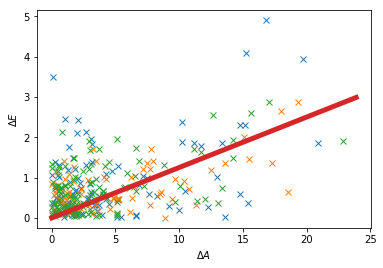
\includegraphics[width=\linewidth]{figures/emb_change.png}
%\end{minipage}%
%\captionof{figure}{Embedding vs adjacency stability on three runs}
%\end{center}

%%%%%%%%%%%%%%%%%%%%%%%%%%%%%%%%%%%%
\chapter{Conclusion}

Building off of prior models, we were able to construct a dynamic model of social networks that exhibits notable real-world properties, including some that to our knowledge have not been studied on Schelling networks or dynamic models in general. Using this model as a training baseline, we extend and improve existing work to construct a dynamic graph-convolutional graph embedding system that significantly outperforms most existing embedding systems. \\

Our dynamic network model is a synthesis of the Barabási–Albert model of preferential attachment, the Apt-Markakis model of product diffusion, and Schelling's model of segregation. We make minor changes to each to get them to work together and to adapt Schelling's model to networks. We then go on to show numerous properties of this synthetic model, including scale-free and small-world structure. In the course of examining small-world behavior we stumbled upon another emergent property of our network: densification. This is an especially interesting phenomena in that to our knowledge it has not been shown in the context of Schelling network models, which is the source of it in our synthetic model. We then go on to study self-similarity of our model, another area which to our knowledge has been little-studied in network analysis. \\

Building on prior work and our synthetic model, we go on to construct a node embedding system. The embedding system is a graph-convolutional autoencoder whose input is the adjacency information augmented by a random walk performed at each epoch. This walk augmentation allowed for significantly more topological information to be used in embedding a given node, and introduced a degree of randomness to encourage the encoder to generate good embeddings. We make heavy use of standard and graph convolutions in our model to keep the network size manageable and to take full advantage of the graph's topology. We then use hinge loss for reconstruction and a cosine loss to maximize distance between non-adjacent nodes and train the model via SGD or Adam, depending on the dataset. Using this method we were able to significantly outperform existing systems both on clustering performance and embedding stability. \\

On the CORA dataset we were able to achieve a classification accuracy of 0.692 using only simple k-means clustering on our embeddings, an accuracy that is on par with decision trees explicitly trained on the data for the classification task. On our synthetic model k-means clustering approached the modularity of partitions discovered by the Louvain algorithm, and on all tested datasets our embeddings were extremely stable over time, often by more an order of magnitude than the adjacency matrices. Our model also trains faster on larger datasets than other models, a feature we ascribe to our heavy use of convolution. \\

All told, both our systems exceeded our expectations in numerous ways. Our dynamic network model exhibited two emergent behaviors we did not expect: self-similarity and densification, both of which are found in real-world networks. We planned only to match performance of existing embedding systems with ours, but were able to outperform them even on static graphs, often by significant margins. \\

\section{Ethics and Legality}

Our work does not in and of itself have any major ethical or legal considerations and we did not see anything in the ethics checklist applicable to our project. While we did use some real-world datasets, these are all standard datasets that had been anonymized before we even downloaded them and have been widely used across the field. While an argument could be made that the entire field of social media analytics and more specifically node embedding has uncomfortable applications towards real-world users as highlighted by Facebook's recent troubles, our particular project is no more or less dubious than any other in the field. The social network model is particularly innocuous, as there is hardly any application in which it could have implications on personal privacy or any other such concern. \\

\section{Future Work}

There are numerous areas of future work we could imagine for our project, from extending and applying the current work to solving issues we could not find elegant solutions to. \\

\subsection{The Network Model}

While we were very happy with how our model behaved, the edge saturation problem remains an unsolved issue. We believe that addressing this would require a fundamentally different translation of Schelling's model to the network space, or at the very least the introduction of another model that discourages edge formation. We view the latter as the less elegant approach as our model is already a synthesis of three models: throwing another on it would hardly be desirable. \\

Another future direction would be closer study of self-similarity. We were unable to draw conclusive evidence of self-similarity despite strong indications of its presence. A further examination of this on the existing model would no doubt shine further light on the model properties, and could lead to studying how to tune the model to promote stronger self-similarity. \\

\subsection{The Embedding System}

Again, we were quite happy with our network model an don't have any major issues that remain to be addressed. That being said, two natural extensions exist in our view, both related to the network structure itself: multimodal variational autoencoders and RNNs. \\

A multimodal variational autoencoder such as the one proposed by Wu \cite{wu2018multimodal} seems like it would be a natural choice to model our social networks, as it is plausible to imagine each community as a single modality. This would intuitively map each node to a given community to and then optimize their placement within whichever community they're a member of. This approach does have numerous drawbacks however: the number of communities would need to be known in advance and it would be difficult to extend to overlapping community membership. Regardless, we view this as a promising direction if only for simple, non-overlapping networks. \\

RNN architectures are another natural extension due to their ability to capture time-series information. Our model preserves the previous step's information by effectively initializing the network to the same weights, but RNNs carry information about prior states and networks which could capture trends our model is unable to. We view this as a more useful direction for future research than MVAEs as they are more well-studied and more promising for more complex datasets. \\

An application that warrants further study is the one we touched on earlier: taking a closer look at node trajectories. We posited that examining a node's trajectory in the embedding space over time could have real predictive power in predicting future community membership or interest, and would like to study that with more detail. Doing so would require large computational power and a time-series annotated dataset, which may not be realistically achievable with our system, but the prospects are nonetheless exciting as to our knowledge no graph-based techniques have been used for this outside recommender systems. \\

%% bibliography

\bibliographystyle{unsrt}
\bibliography{bibliography} 


\end{document}
